\documentclass[11pt]{beamer}
\usetheme{Rochester}

\usepackage[dutch]{babel}

\usepackage[utf8]{inputenc}
\usepackage[T1]{fontenc}

\title{Introductie Android Studio}
\subtitle{Apps ontwikkelen voor het Android Platform}
%\logo{\includegraphics{bogermanlogo}}
%\institute{}
\date{Versie: \today}
%\subject{}
%\setbeamercovered{transparent}
\setbeamertemplate{navigation symbols}{}

\begin{document}
\maketitle

\begin{frame}
\frametitle{Waarom Android Studio?}
Alles wat je nodig hebt in \'e\'en pakket
\begin{itemize}
\item Project management
\item Code editor
\item Layout viewer
\item Android Emulator
\end{itemize}
\end{frame}

\begin{frame}
\frametitle{Een nieuw project maken}
\begin{figure}
\centering
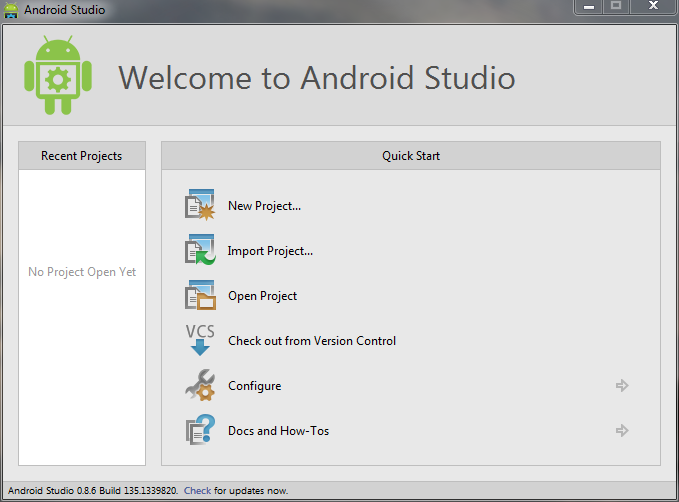
\includegraphics[height=.9\textheight]{./newproject1}
\label{fig:newproject1}
\end{figure}
\end{frame}

\begin{frame}
\frametitle{Een nieuw project maken}
\begin{figure}
\centering
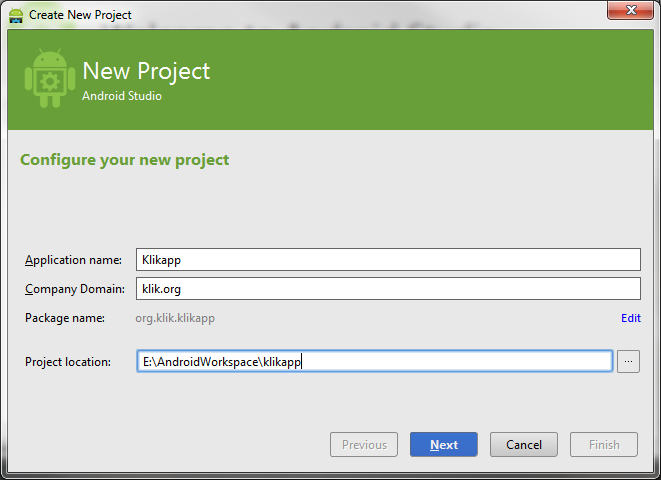
\includegraphics[height=.9\textheight]{./newproject2}
\label{fig:newproject2}
\end{figure}
\end{frame}

\begin{frame}
\frametitle{Android versie kiezen}
\begin{figure}
\centering
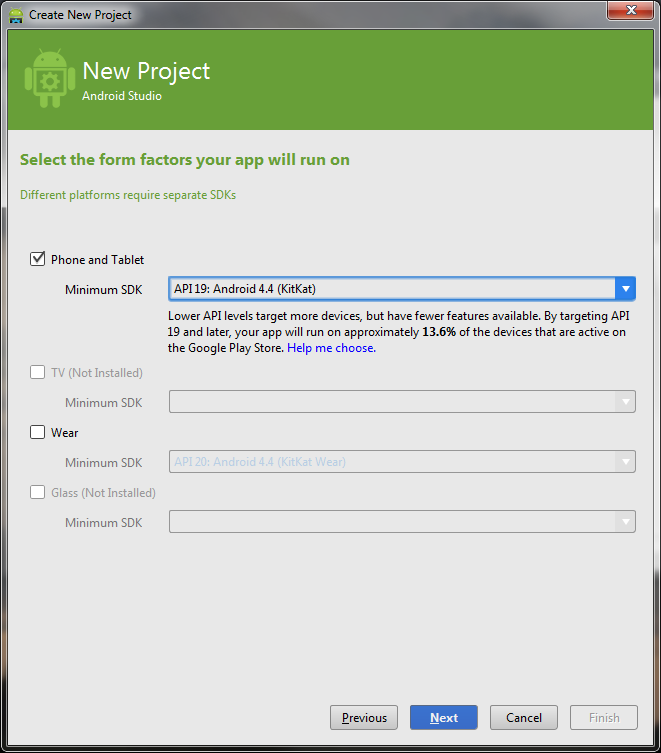
\includegraphics[height=.9\textheight]{./newproject3}
\label{fig:newproject3}
\end{figure}
\end{frame}

\begin{frame}
\frametitle{Android versie kiezen}
\begin{figure}
\centering
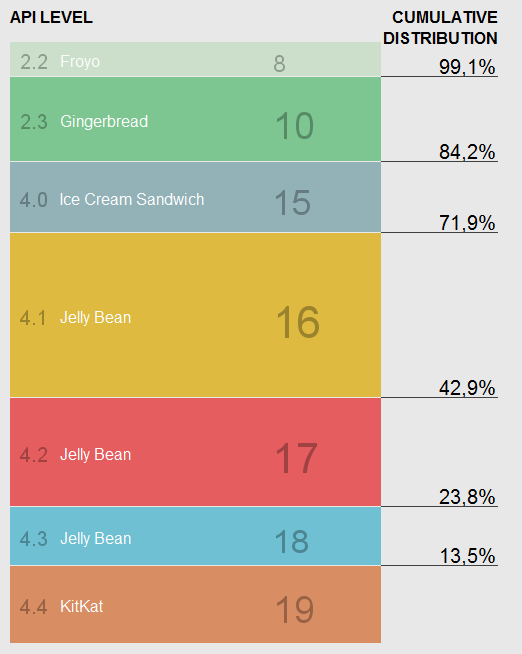
\includegraphics[height=.75\textheight]{./apilevel1}
\caption{29 september 2014}
\label{fig:apilevel1}
\end{figure}
\end{frame}

\begin{frame}
\frametitle{Start Activity (index pagina)}
\begin{figure}
\centering
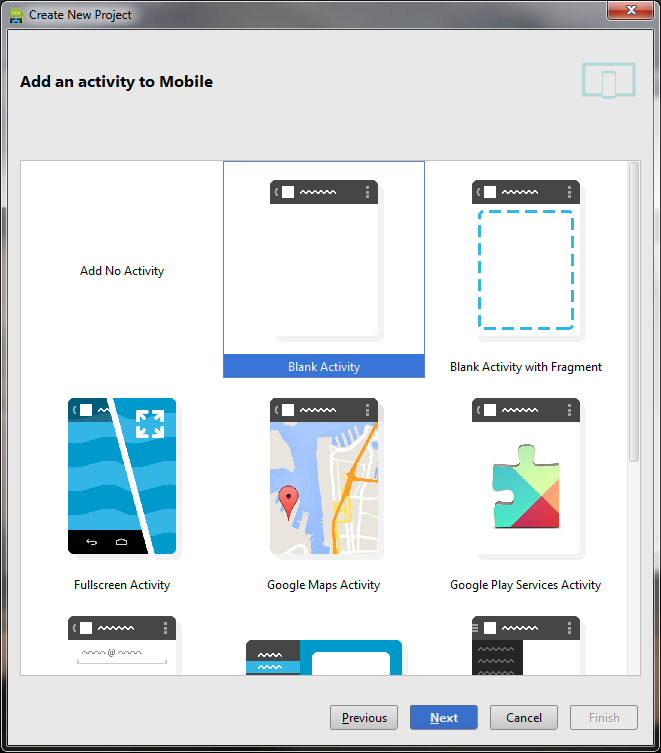
\includegraphics[height=.9\textheight]{./newactivity}
\label{fig:newactivity1}
\end{figure}
\end{frame}



\begin{frame}
\frametitle{Gegevens invullen van de activity}
\begin{figure}
\centering
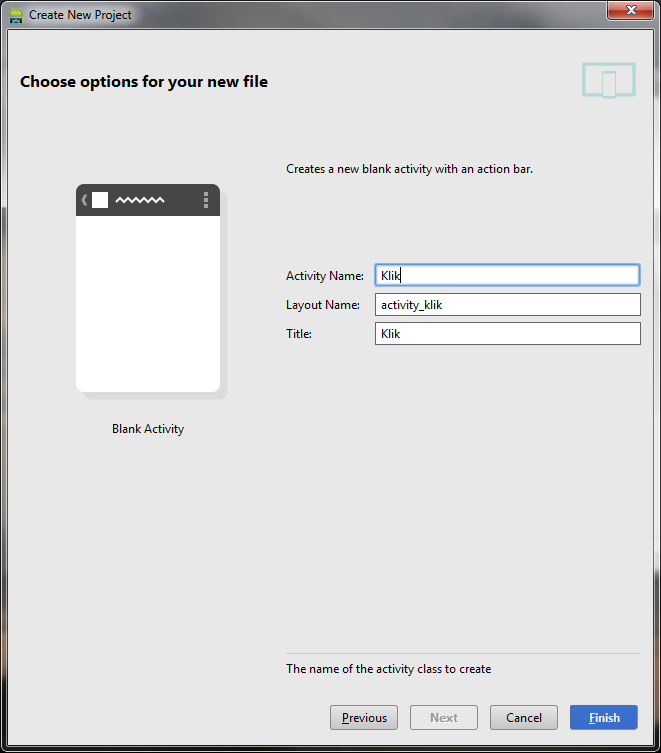
\includegraphics[height=.9\textheight]{./newproject4}
\label{fig:newproject4}
\end{figure}
\end{frame}


\begin{frame}
\frametitle{Het hoofdscherm}
\begin{figure}
\centering
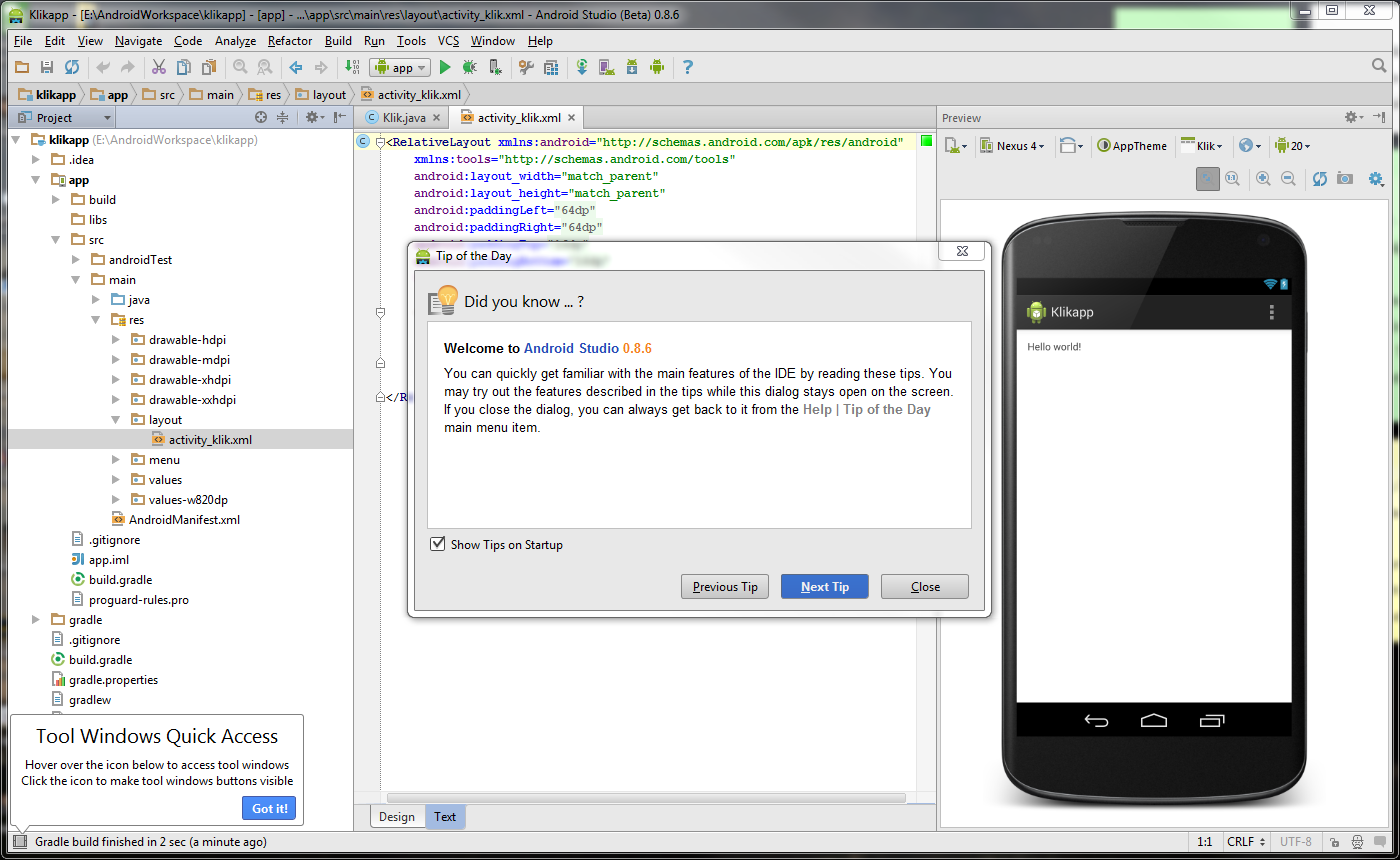
\includegraphics[width=1.0\linewidth]{./asinterface1}
\label{fig:asinterface1}
\end{figure}
\end{frame}

\begin{frame}
\frametitle{Mappen structuur - links}
\begin{figure}
\centering
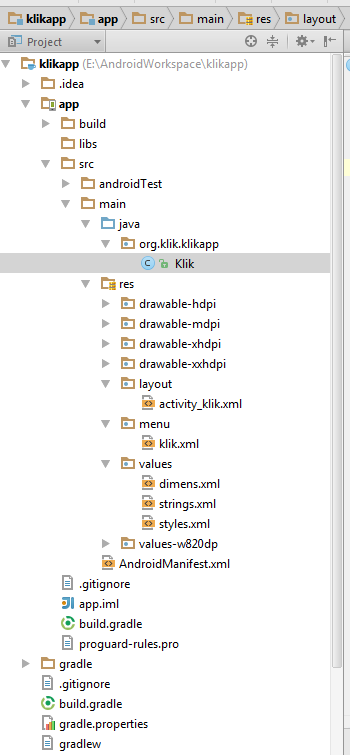
\includegraphics[height=.9\textheight]{./asinterface2}
\label{fig:asinterface2}
\end{figure}
\end{frame}

\begin{frame}
\frametitle{Code editor - midden}
\begin{figure}
\centering
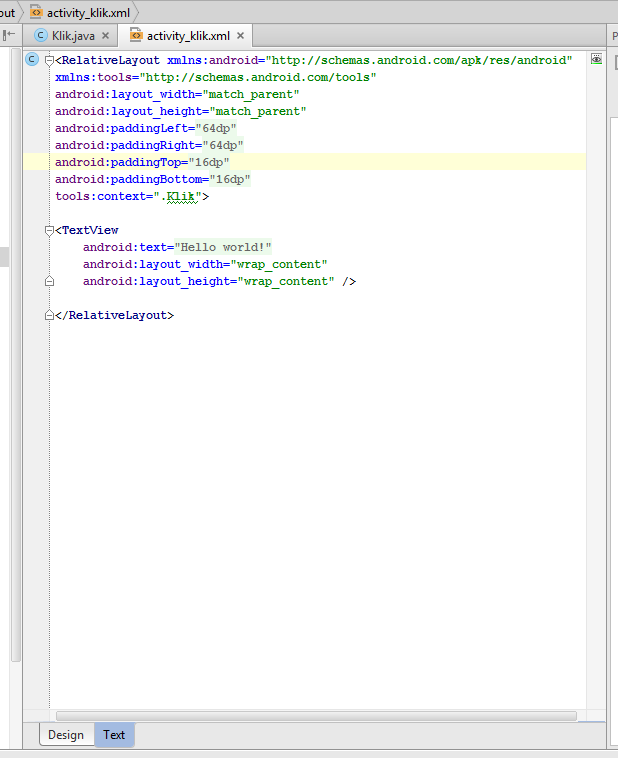
\includegraphics[height=.9\textheight]{./asinterface3}
\label{fig:asinterface3}
\end{figure}
\end{frame}

\begin{frame}
\frametitle{Live layout - rechts}
\begin{figure}
\centering
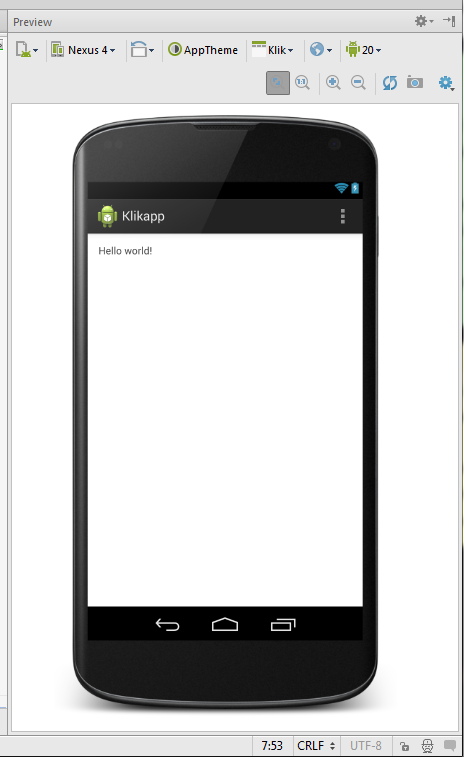
\includegraphics[height=.9\textheight]{./asinterface4}
\label{fig:asinterface4}
\end{figure}
\end{frame}

%Nieuwe activiteit maken
\begin{frame}
\frametitle{Een nieuwe activiteit maken} \pause
\begin{figure}
\centering
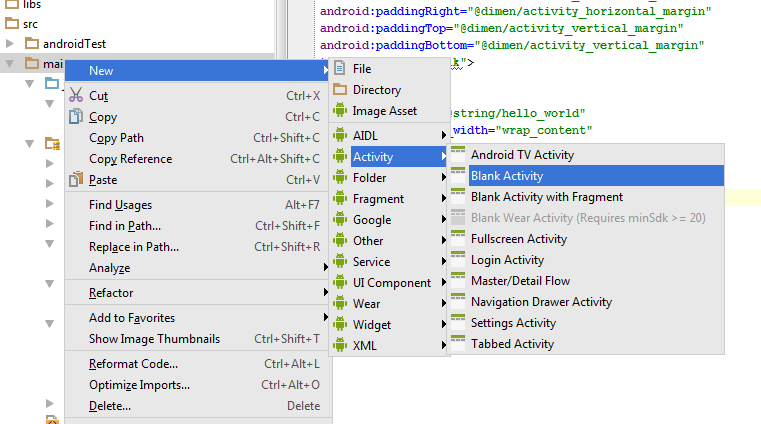
\includegraphics[width=1.0\linewidth]{./newactivity2}
\label{fig:newactivity2}
\end{figure}
\end{frame}

\begin{frame}
\frametitle{Een nieuwe activiteit maken}
\begin{figure}
\centering
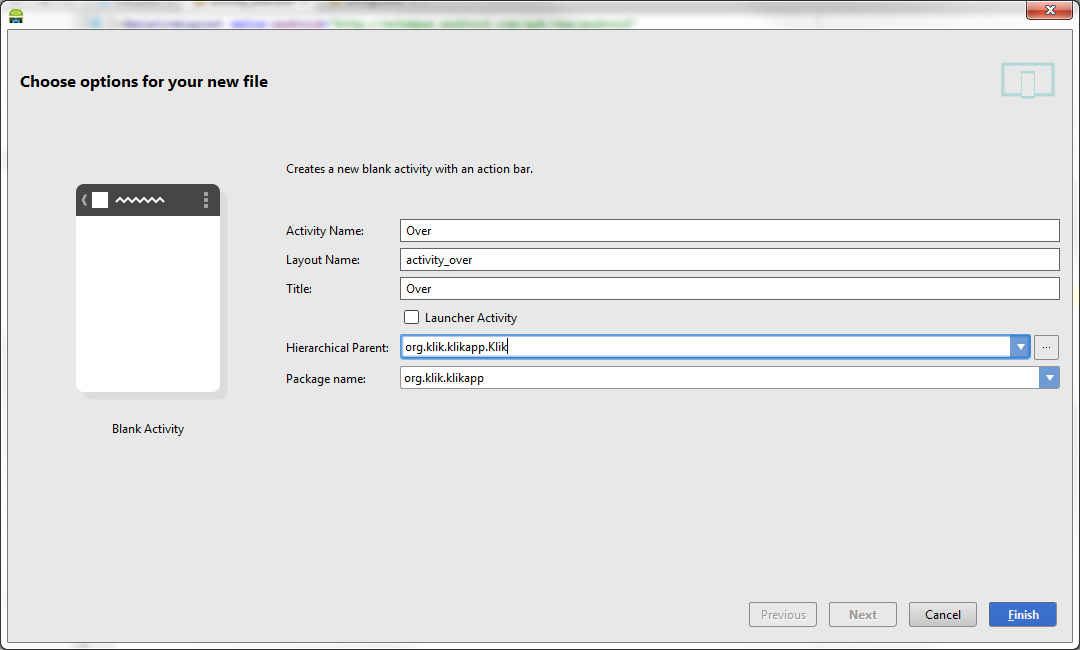
\includegraphics[width=1.0\linewidth]{./newactivity3}
\label{fig:newactivity3}
\end{figure}
\end{frame}


\begin{frame}
\frametitle{Tekst aanpassen}
\begin{figure}
\centering
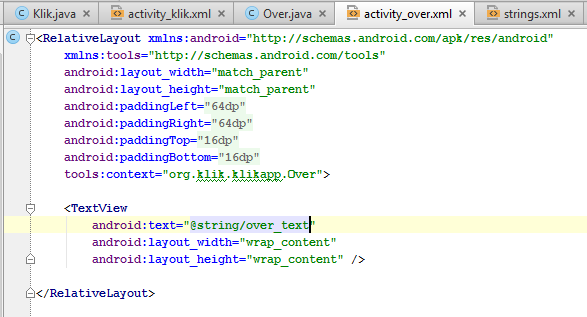
\includegraphics[width=1.0\linewidth]{./stringediting2}
\label{fig:stringediting1}
\end{figure}
\end{frame}

\begin{frame}
\frametitle{Tekst aanpassen}
\begin{figure}
\centering
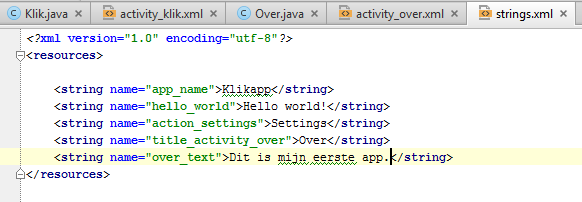
\includegraphics[width=1.0\linewidth]{./stringediting}
\label{fig:stringediting2}
\end{figure}
\end{frame}

\begin{frame}
\frametitle{Tekst aanpassen}
\begin{figure}
\centering
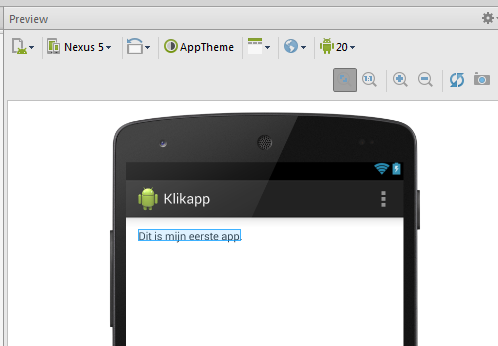
\includegraphics[height=.9\textheight]{./stringediting3}
\label{fig:stringediting3}
\end{figure}
\end{frame}

%Knop toevoegen

\begin{frame}
\frametitle{Een knop toevoegen}
\begin{figure}
\centering
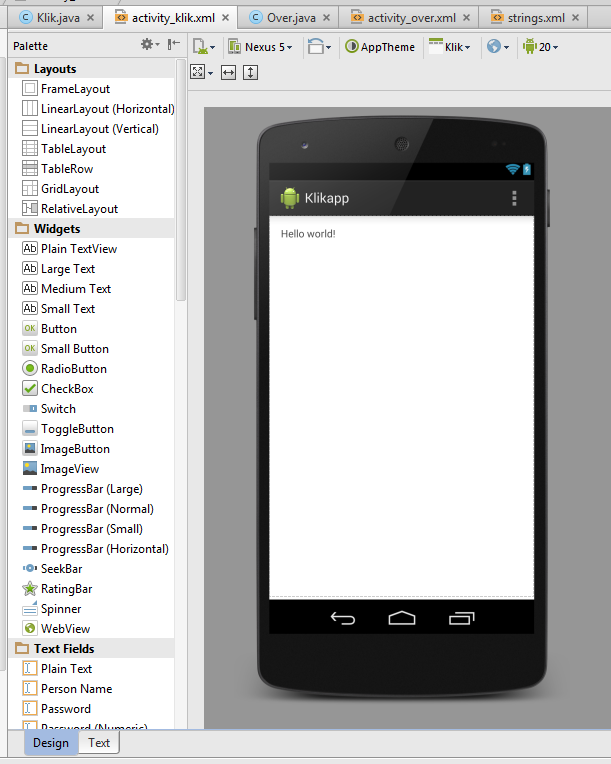
\includegraphics[height=.9\textheight]{./addbutton1}
\label{fig:addbutton1}
\end{figure}
\end{frame}

\begin{frame}
\frametitle{Een knop toevoegen via design}
\begin{figure}
\centering
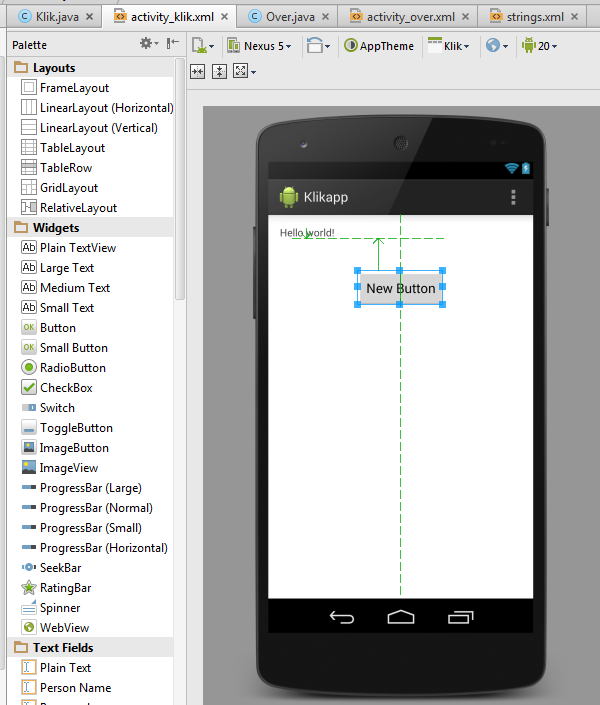
\includegraphics[height=.9\textheight]{./addbutton2}
\label{fig:addbutton2}
\end{figure}
\end{frame}

\begin{frame}
\frametitle{Een knop toevoegen de knop een naam en tekst geven}
\begin{figure}
\centering
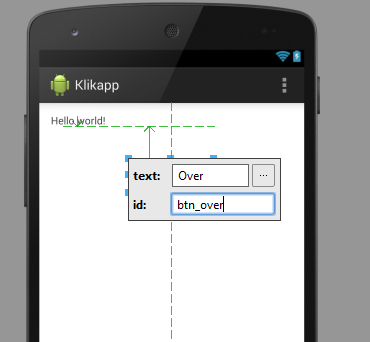
\includegraphics[height=.9\textheight]{./addbutton3}
\label{fig:addbutton3}
\end{figure}
\end{frame}

\begin{frame}
\frametitle{De knop tekst op de de juiste plaats zetten}
\begin{figure}
\centering
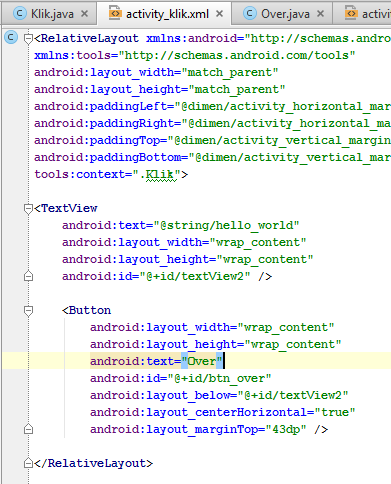
\includegraphics[height=.9\textheight]{./addbutton4}
\label{fig:addbutton4}
\end{figure}
\end{frame}

\begin{frame}
\frametitle{De knop tekst op de de juiste plaats zetten}
\begin{figure}
\centering
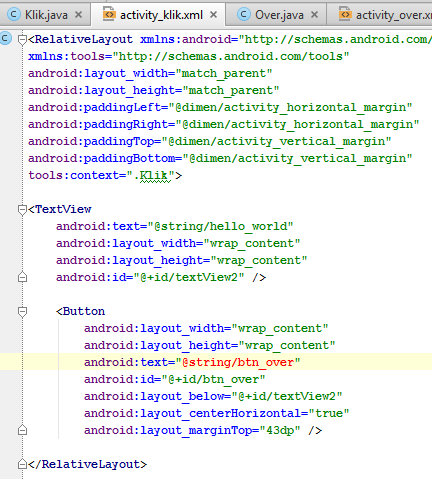
\includegraphics[height=.9\textheight]{./addbutton5}
\label{fig:addbutton5}
\end{figure}
\end{frame}

\begin{frame}
\frametitle{De knop tekst op de de juiste plaats zetten}
\begin{figure}
\centering
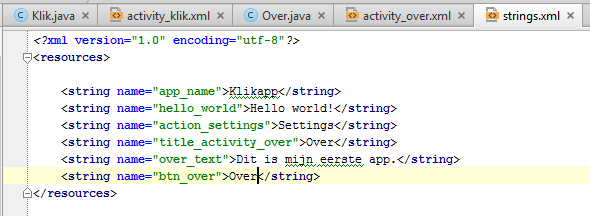
\includegraphics[width=1.0\linewidth]{./addbutton6}
\label{fig:addbutton6}
\end{figure}
\end{frame}

%Intents maken

\begin{frame}
\frametitle{Een actie aan de knop toevoegen}
\begin{figure}
\centering
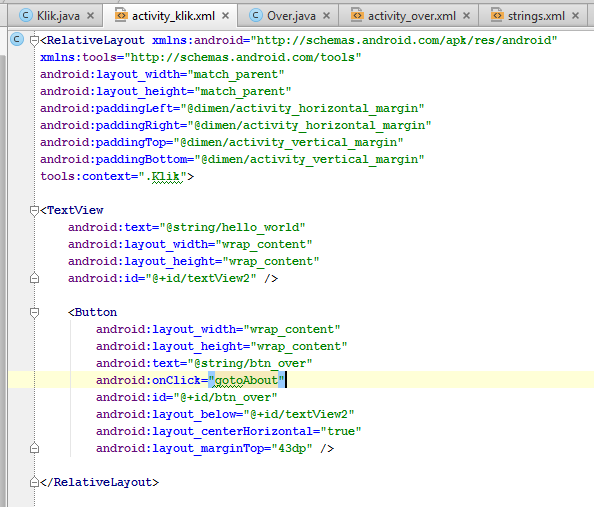
\includegraphics[height=.9\textheight]{./intent1}
\label{fig:intent1}
\end{figure}
\end{frame}

\begin{frame}
\frametitle{Een actie aan de knop toevoegen}
\begin{figure}
\centering
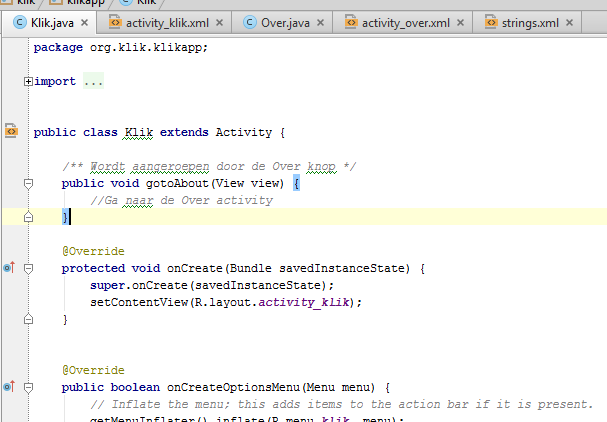
\includegraphics[height=.9\textheight]{./intent2}
\label{fig:intent2}
\end{figure}
\end{frame}

\begin{frame}
\frametitle{Een Intent aan de actie koppelen}
Bestand: \textit{Klik.java}
\begin{figure}
\centering
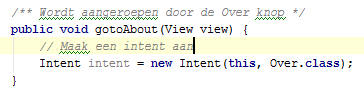
\includegraphics[width=.9\linewidth]{./intent3}
\label{fig:intent3}
\end{figure}
\end{frame}

\begin{frame}
\frametitle{De andere activiteit starten}
Bestand: \textit{Klik.java}
\begin{figure}
\centering
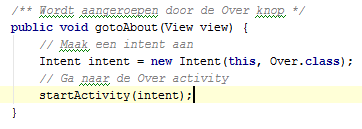
\includegraphics[width=.9\linewidth]{./intent4}
\label{fig:intent4}
\end{figure}
\end{frame}


%Volgende les:
%Virtuele telefoon maken




%Frame work
%\begin{frame}
%
%\begin{columns}
%	\begin{column}{.5\textwidth}
%
%	\end{column}
%	\begin{column}{.5\textwidth}
%
%	\end{column}
%\end{columns}
%
%\end{frame}


\end{document}